
\section{Sample growth}

The samples were grown and initially characterised by Prof. Takeuchi's group in Sendai University, Japan in May 2009 using the floating zone technique. Here powders of the correct stoichiometry are compacted into a rod and fed slowly through a furnace where it becomes a viscous melt. The melt solidifies epitaxially on a seed crystal with impurities held in the melt portion of the crystal which gradually moves up, along the rod until it reaches the end of the rod and the growth is over. The end portion, containing the impurities is then removed. Similar samples have already been extensively studied through \ac{ARPES} and \ac{STM} by memebers of the Sendai group~\cite{Wise2009, Wise2008, Kondo2007, Kondo2005, Kondo2010, Kondo2009, Kondo2006, Kondo2007}.

Table~\ref{Tab:ExpH:SampleGrowthDetails} lists the nominal stoichiometries for the sample growth as well as the annealing conditions. Also listed are the \emph{nominal} \Tc values for the source crystals which are used in the naming, the actual measured \Tc values of individual samples for the purposes of doping determination are slightly different due to different definitions of \Tc\footnote{The source crystals were defined based on the zero value \Tc, the \Tc for doping purposes is defined as the mid-point of the transition with an error based on the difference between the mid-point and the zero-point.}.
% \begin{table}
%     \begin{center}
%            \caption{Doping as determined by the Tallon relation, the Ando relation and scaling to \ac{TL2201} data as described in the method section.}
%         \begin{tabular}[htbp]{lrrrr}
% \toprule
% Sample	& \Tc ($K$)   & $p_{\textrm{Tallon}}$	& $p_{\textrm{Ando}}$	& $p_{\textrm{Tl}}$	\\
% \midrule
% B00KOD1A	& $0.0\pm1.0$	& $0.270\pm0.003$	& $0.223\pm0.002$	& $0.311\pm0.004$	\\
% B07KOD2		& $11\pm3.8$	& $0.252\pm0.013$	& $0.212\pm0.008$	& $0.271\pm0.013$	\\
% B16KOD1A	& $17\pm1.0$	& $0.240\pm0.004$	& $0.206\pm0.002$	& $0.249\pm0.004$	\\
% B30KOD3		& $29\pm0.5$	& $0.209\pm0.003$	& $0.188\pm0.002$	& $0.209\pm0.003$	\\
% B32KOP1		& $36\pm1.0$	& $0.160\pm0.018$	& $0.160\pm0.010$	& $0.160\pm0.018$	\\
% B32KOP4		& $35\pm2.0$	& $0.178\pm0.026$	& $0.170\pm0.015$	& $0.178\pm0.026$	\\
% B30KUD3		& $32\pm1.0$	& $0.123\pm0.008$	& $0.139\pm0.005$	& $0.123\pm0.008$	\\
% B28KUD3A	& $31.5\pm1.0$	& $0.121\pm0.008$	& $0.138\pm0.004$	& $0.121\pm0.008$	\\
% \bottomrule
%         \label{Tab:ExpH:Dopings}
%         \end{tabular}
%     \end{center}
% \end{table}
Figure~\ref{Fig:ExpH:Dopings} shows the the normalised \Tc vs. the doping by each of the three techniques outlined in the methods section. The dopings of the crystals range from $p=0.12$ to $p=0.31$ holes per Cu atom with significant discrepencies between the three methods. The Ando method gives the tightest spread of dopings, whilst comparing the \ac{TL2201} data gives the widest. The Tallon data sits between the two. For the purpose of this thesis, the Tallon method doping will be used, with the other data being considered when determining errors.


\begin{table}
    \begin{center}
           \caption{Growth details for the \ac{BSCO} samples. OD, OP and UD stand for over, optimally and under doped respectively. $T_c$ values are nominal.}
        {\small \begin{tabular}[htbp]{lllllllll}
\toprule
\multicolumn{6}{c}{Nominal composition} & & & \\
Bi  & Pb  & Sr  & La  & Cu  & O   & $T_c$   & Reg.  & Annealing conditions \\
\midrule
1.72    & 0.38  & 1.85  & 0.0   & 1.0   & 6+d   & $<$2  & OD    & \unit{400}{\celsius}, \unit{96}{\hour} in \unit{2.5}{\textrm{atm.}} O$_2$ \\
1.72    & 0.38  & 1.85  & 0.0   & 1.0   & 6+d   & 7     & OD    & \unit{750}{\celsius}, \unit{24}{\hour} in air \\
1.72    & 0.38  & 1.85  & 0.0   & 1.0   & 6+d   & 16    & OD    & \unit{550}{\celsius}, \unit{72}{\hour} in flowing N$_2$ \\
1.35    & 0.85  & 1.47  & 0.38  & 1.0   & 6+d   & 30    & OD    & As grown \\
1.35    & 0.85  & 1.47  & 0.38  & 1.0   & 6+d   & 32    & OP    & \unit{650}{\celsius}, \unit{72}{\hour} in flowing N$_2$ \\
1.2     & 0.90  & 1.30  & 0.55  & 1.0   & 6+d   & 30    & UD    & As grown \\
1.2     & 0.90  & 1.30  & 0.55  & 1.0   & 6+d   & 28    & UD    & \unit{650}{\celsius}, \unit{72}{\hour} in flowing N$_2$ \\
\bottomrule
        \label{Tab:ExpH:SampleGrowthDetails}
        \end{tabular}}
    \end{center}
\end{table}

The samples are named according the convention,
\begin{quote}
\code{B<Tc>K<Region><Crystal No.><Sample No.>}
\end{quote}
so for example `B00KOD2A' refers to the sample `A' taken from the crystal `B00KOD2' --- the second overdoped crystal with a $T_c$ of $\unit{0}{K}$.

\section{Size determination}

Thicknesses were determined for some of the samples using the \ac{FIB} or the optical microscope as described in the methods section. The thicknesses used to calculate abolute values of $R_H$ are listed in table~\ref{Tab:ExpH:Thicknesses}. Thicknesses for all measured samples are detailed in Appendix~\ref{Sec:AppSampleSizes}. \ac{FIB} results are given for areas as close to the two voltage contacts that were visible in the scans. As can be seen in the example scan shown in figure~\ref{Fig:ExpH:FIBExample}, there is some variation in the depth along the sample length. Measurements are therefore taken as close to the voltage legs as possible and whre appropriate suitable errors are estimated.
\begin{figure}[htbp]
	\begin{center}
		\includegraphics[scale=0.9]{Chapter-HallBSCO/Figures/FIBExamples/FIBExamples}
		\caption{Top shows an image composited from several \ac{FIB} scans along the length of sample B00KOD1a, with bottom right showning a detail of the right voltage leg.  bottom left shows an oblique top down view of sample B30KOD3.}
		\label{Fig:ExpH:FIBExamples}
	\end{center}
\end{figure}

The two scans shown are of good quality, however for the purpose of estimating errors in the thickness some of the scans presented problems. Samples B26KOD1a, B28KUD3a, B30KOD2 and B30KUD3 were obscured with the grease applied as part of the pulsed field measurements. Other samples were not correctly earthed such as B28KUD3b which made the images dark, whilst samples B07KOD2 and B32KOP3 were very flakey under close scrutiny. A scan of B30KOD3 showed that it was partially split in the ab plane which may contribute to systematic error in thickness estimate. In all these cases, the esimate in the thickness error was adjusted accordingly to compensate. A more comprehensive set of \ac{FIB} scans, including images of the split in the layers can be found in Appendix~\ref{Appendix:FIBScans}.

The oblique view of B30KOD3 in figure~\ref{Fig:ExpH:FIBExample} shows a clear misalignment of the voltage legs to thr right of the image. This illustrates why it is necessary to take both positive and negative field sweeps in order to seperate the magnetoresistance from the Hall components.

\begin{table}
    \begin{center}
           \caption{Sample measurements as determined by optical microscope measurements and thickness as determined by \ac{FIB}. Samples highlighted in grey were used for determining absolute values of $R_H$. A and B refer to each of the two contacts visible to the \acs{FIB} scan. Measurements are in micrometres.}
        \begin{tabular}[htbp]{lrrrrr}
\toprule
	& \multicolumn{3}{c}{Optical}			& \multicolumn{2}{c}{\acs{FIB}}		\\
Sample  & Length	& Width		& Thick.	& Contact A    & Contact B    		\\

\midrule
\cellcolor[gray]{0.9}B00KOD1A	& \cellcolor[gray]{0.9}$781\pm123$	& \cellcolor[gray]{0.9}$157\pm49$	& \cellcolor[gray]{0.9}N/A		& \cellcolor[gray]{0.9}$45\pm1$	& \cellcolor[gray]{0.9}$50\pm5$	\\
B00KOD1B	& $627\pm49$	& $196\pm44$	& $39\pm5$ 	& $43\pm1.5$	& $45\pm1.5$	\\
B07KOD1		& $1277\pm74$	& $392\pm49$	& $29\pm10$	& N/A		& N/A		\\
\cellcolor[gray]{0.9}B07KOD2		& \cellcolor[gray]{0.9}$1061\pm69$	& \cellcolor[gray]{0.9}$333\pm74$	& \cellcolor[gray]{0.9}N/A		& \cellcolor[gray]{0.9}$20\pm5$ 	& \cellcolor[gray]{0.9}$30\pm1$ 	\\
\cellcolor[gray]{0.9}B16KOD1A	& \cellcolor[gray]{0.9}$795\pm34$	& \cellcolor[gray]{0.9}$299\pm34$	& \cellcolor[gray]{0.9}N/A		& \cellcolor[gray]{0.9}$24\pm1$ 	& \cellcolor[gray]{0.9}$24\pm1$ 	\\
B16KOD2A	& $358\pm29$	& $172\pm54$	& $9\pm1$ 	& N/A		& N/A		\\
B16KOD3		& $1122\pm44$	& $368\pm83$	& N/A		& $25\pm2$ 	& $24\pm2$ 	\\
B30KOD1	 	& $436\pm34$	& $250\pm44$	& $21\pm2$ 	& N/A		& N/A		\\
B30KOD2		& $344\pm44$	& $137\pm29$	& $20\pm5$ 	& $15\pm4$	& $15\pm4$	\\
\cellcolor[gray]{0.9}B30KOD3 	& \cellcolor[gray]{0.9}$255\pm49$	& \cellcolor[gray]{0.9}$98\pm25$ 	& \cellcolor[gray]{0.9}N/A		& \cellcolor[gray]{0.9}$16.5\pm1.5$	& \cellcolor[gray]{0.9}$19\pm1$	\\
\cellcolor[gray]{0.9}B32KOP1 	& \cellcolor[gray]{0.9}$658\pm83$	& \cellcolor[gray]{0.9}$397\pm34$	& \cellcolor[gray]{0.9}N/A		& \cellcolor[gray]{0.9}$6.5\pm1.5$	& \cellcolor[gray]{0.9}$6.5\pm1.5$	\\
B32KOP2		& $441\pm25$	& $226\pm20$	& $10\pm1$ 	& N/A		& N/A		\\
B32KOP3		& $437\pm34$	& $118\pm20$	& N/A		& $6\pm1$ 	& $6\pm1$ 	\\
B32KOP4 	& $427\pm74$	& $137\pm39$	& N/A		& $9\pm3$ 	& $9\pm3$ 	\\
B30KUD1A	& $622\pm49$	& $447\pm25$	& $36\pm3$ 	& N/A		& N/A		\\
B30KUD1B	& $828\pm34$	& $471\pm64$	& $35\pm3$ 	& N/A		& N/A		\\
B30KUD2 	& $545\pm69$	& $152\pm39$	& N/A		& $5 \pm1$ 	& $5 \pm1$ 	\\
\cellcolor[gray]{0.9}B30KUD3 	& \cellcolor[gray]{0.9}$476\pm49$	& \cellcolor[gray]{0.9}$118\pm34$	& \cellcolor[gray]{0.9}N/A		& \cellcolor[gray]{0.9}$7\pm2$ 	& \cellcolor[gray]{0.9}$7\pm2$ 	\\
B28KUD2A	& $657\pm29$	& $250\pm39$	& $11\pm1$ 	& N/A		& N/A		\\
\cellcolor[gray]{0.9}B28KUD3A	& \cellcolor[gray]{0.9}$633\pm49$	& \cellcolor[gray]{0.9}$142\pm34$	& \cellcolor[gray]{0.9}N/A		& \cellcolor[gray]{0.9}$16\pm3$	& \cellcolor[gray]{0.9}$16\pm3$	\\
B28KUD3B	& $653\pm44$	& $216\pm49$	& N/A		& $16\pm3$	& $16\pm3$	\\
\bottomrule
        \label{Tab:ExpH:Thicknesses}
        \end{tabular}
    \end{center}
\end{table}

